\section{Introdução}

\begin{frame}{Sistema Embarcado}
	\begin{itemize}
			\item 	Um sistema embarcado, ou sistema embutido, é um sistema 
			microprocessado no qual o computador é completamente encapsulado
			ou dedicado ao dispositivo ou sistema que ele controla.

			\item Um sistema embarcado realiza um conjunto de tarefas 
			pré-definidas, geralmente com requisitos específicos.

			\item Já que o sistema é dedicado à tarefas específicas, 
			pode-se otimizar o sistema reduzindo tamanho, recursos 
			computacionais e custo do produto.
	\end{itemize}
\end{frame}

\begin{frame}
    \frametitle{Sistema Embarcado}
    \begin{itemize}
        \item Costumam fazer uso de microcontroladores.
        \item É necessário programar os microcontroladores.
        \item Existem alguns ambientes de desenvolvimento que facilitam
        essa tarefa.
	\end{itemize}

\end{frame}

\begin{frame}
	\frametitle{MPLAB-X IDE}
	\begin{figure}[htbp]
		\centering
		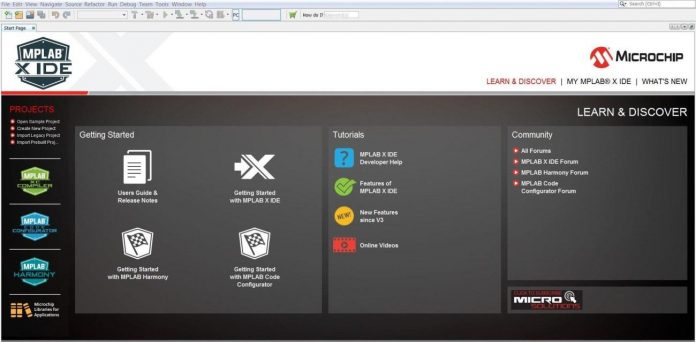
\includegraphics[width=0.9\textwidth]{images/mplab.jpg}
	\end{figure}
\end{frame}

\begin{frame}
	\frametitle{CCS IDE}
	\begin{figure}[htbp]
		\centering
		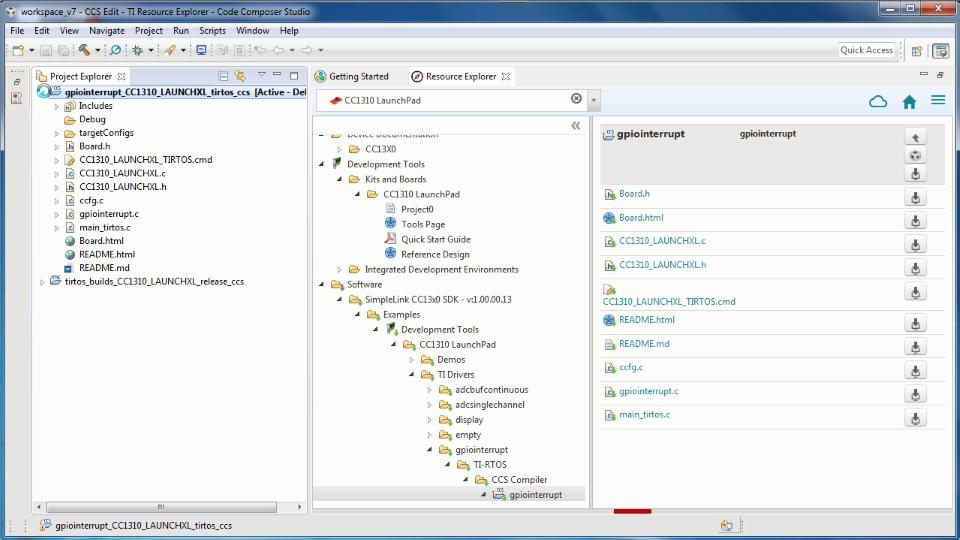
\includegraphics[width=0.9\textwidth]{images/ccs}
	\end{figure}
\end{frame}

\begin{frame}
	\frametitle{Arduino IDE}
	\begin{figure}[htbp]
		\centering
		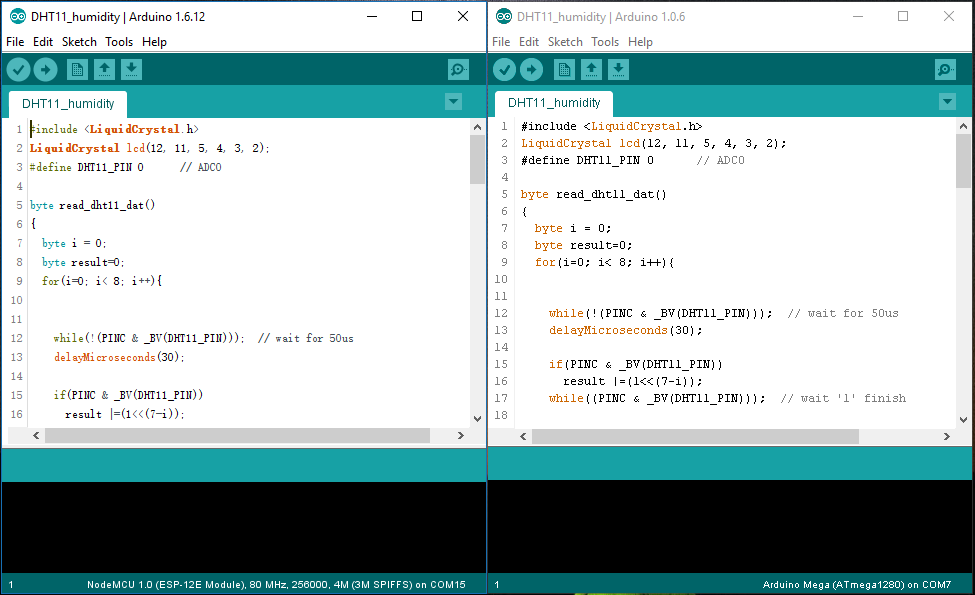
\includegraphics[width=0.8\textwidth]{images/arduino}
	\end{figure}
\end{frame}

\begin{frame}
	\frametitle{Platformio IDE}
	\begin{figure}[htbp]
		\centering
		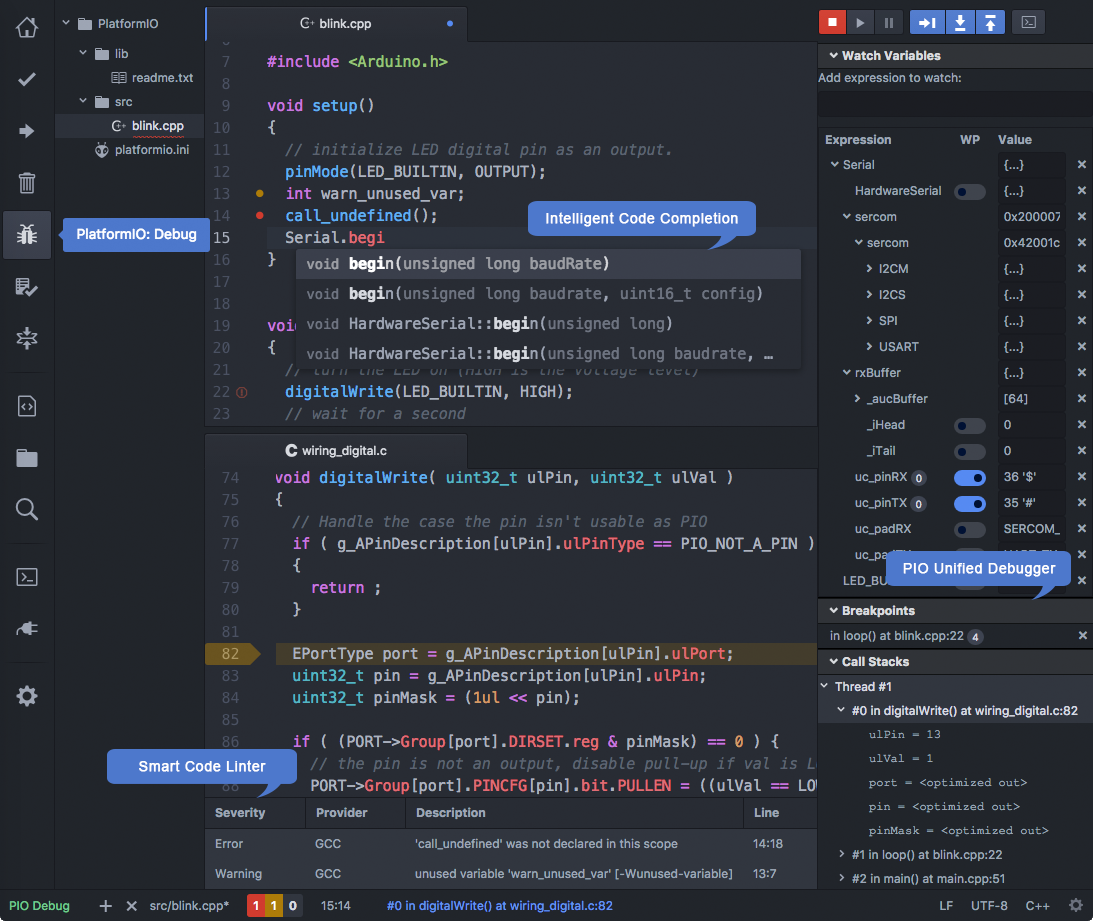
\includegraphics[width=0.8\textwidth]{images/platformio}
	\end{figure}
\end{frame}
